\section{Numerical evidence and validation plan}
\label{sec:experiments}
Figure~\ref{fig:historical-cbc} reuses the two discrepancy comparisons from
the special-session slides. They use $d=64$, construction horizon $N=2^{20}$,
coordinate weights $\gamma_j=j^{-2}$, and sample-size weights $w_n=n$.
The plotted quantity is root expected squared discrepancy at successive
prefix lengths. The lattice comparison contrasts the stored embedded-lattice
vector with the vector selected for the aggregate objective; embedded lattice
construction provides the relevant methodological baseline \cite{CKN06}.
The Kronecker comparison includes the stored CBC vector and the sequences
labeled Richtmyer and Suzuki in the notebook. These are historical
illustrations; they have not been regenerated or independently validated for
this manuscript, and they do not yet test the recent Newo or Kronecker developments.

\begin{figure}[p]
 \centering
 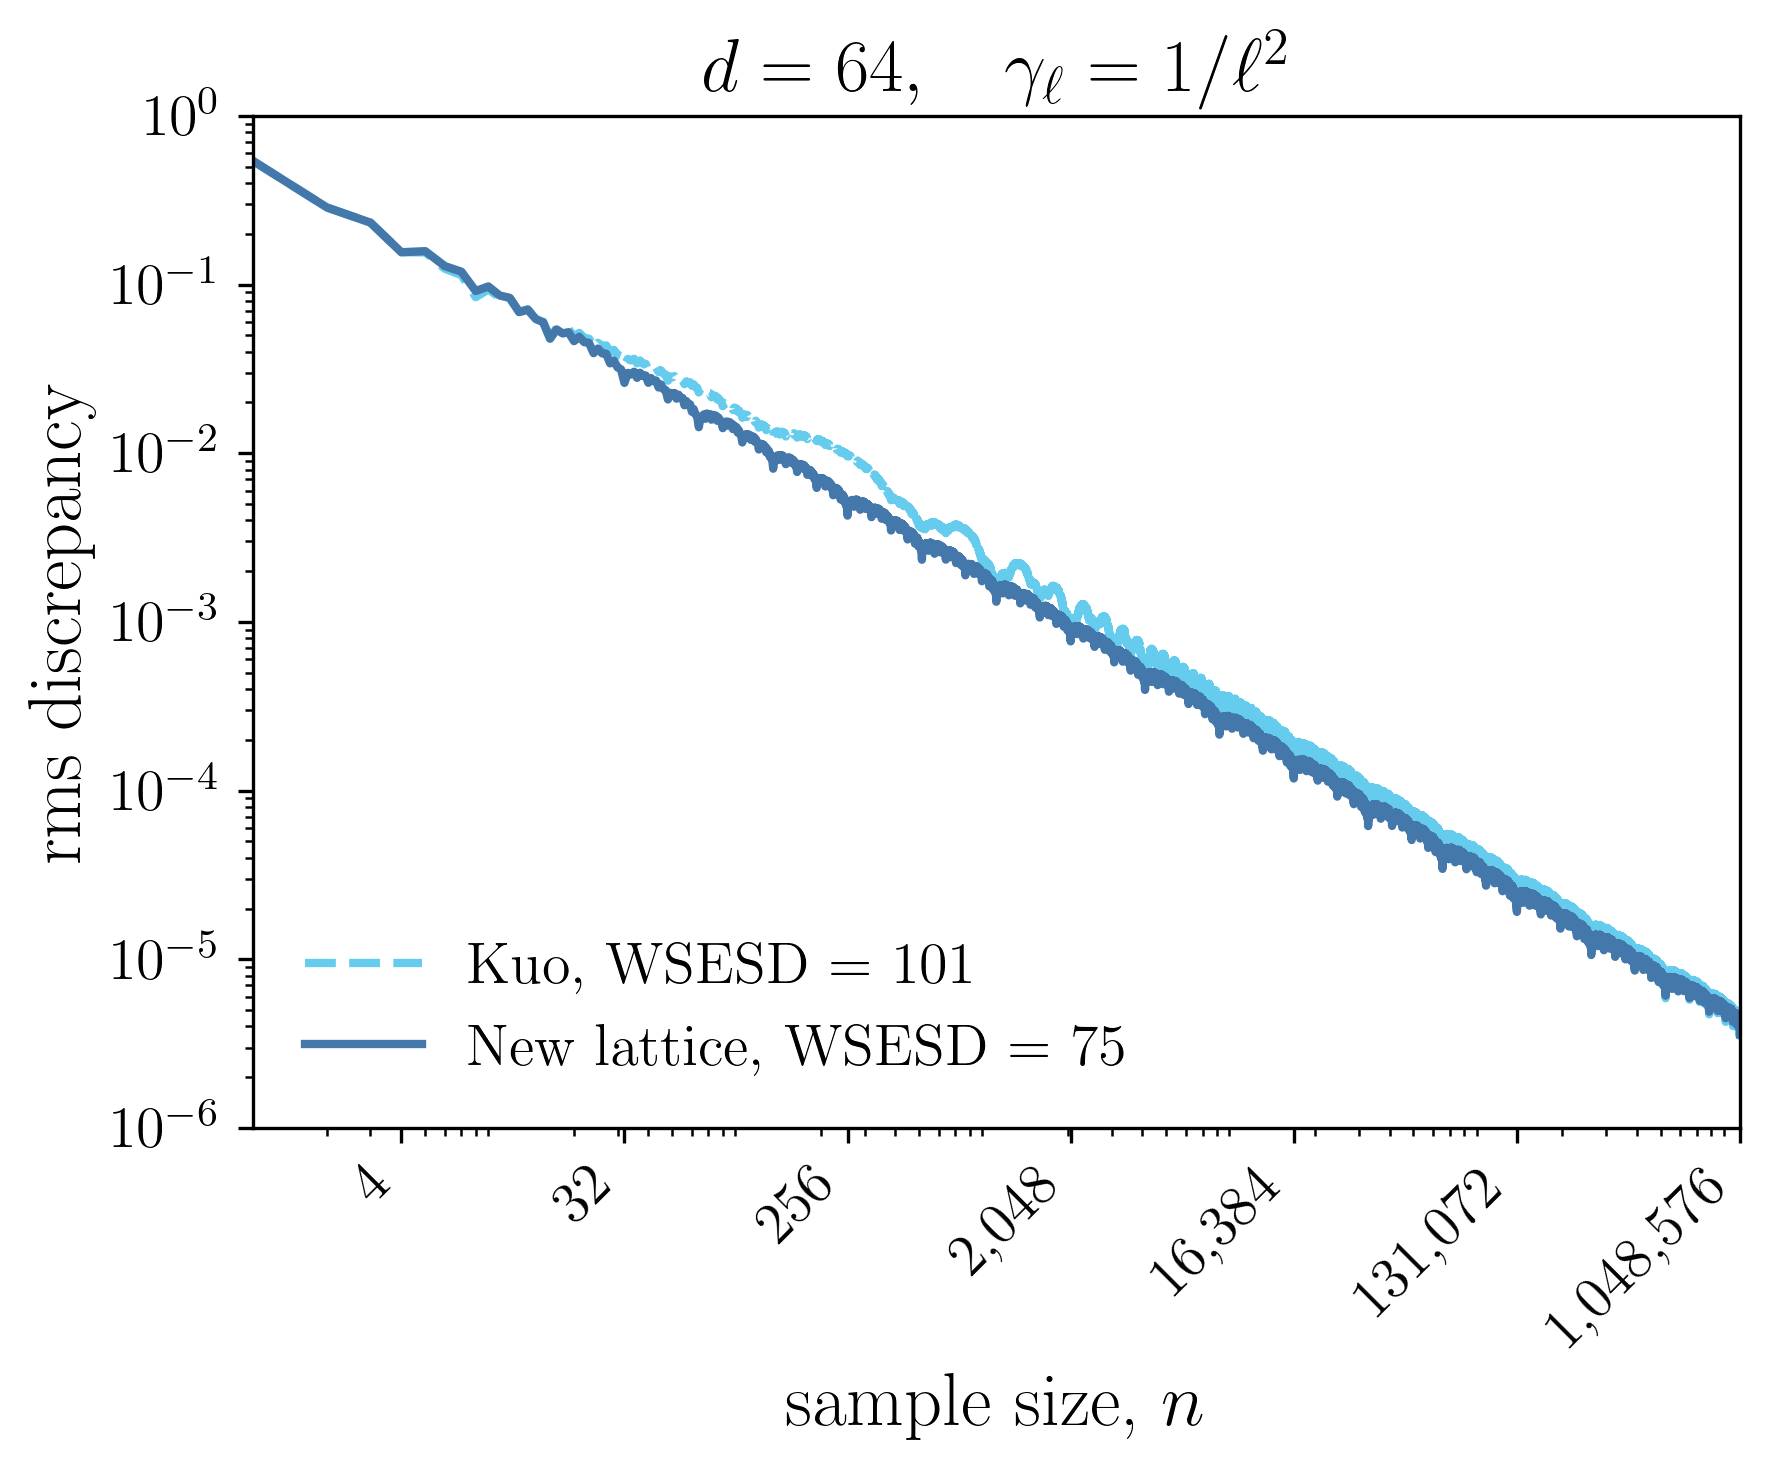
\includegraphics[width=.74\linewidth]{../../notebooks/artifacts/figures/special_d64_lattice_discrepancy.png}\\[1ex]
 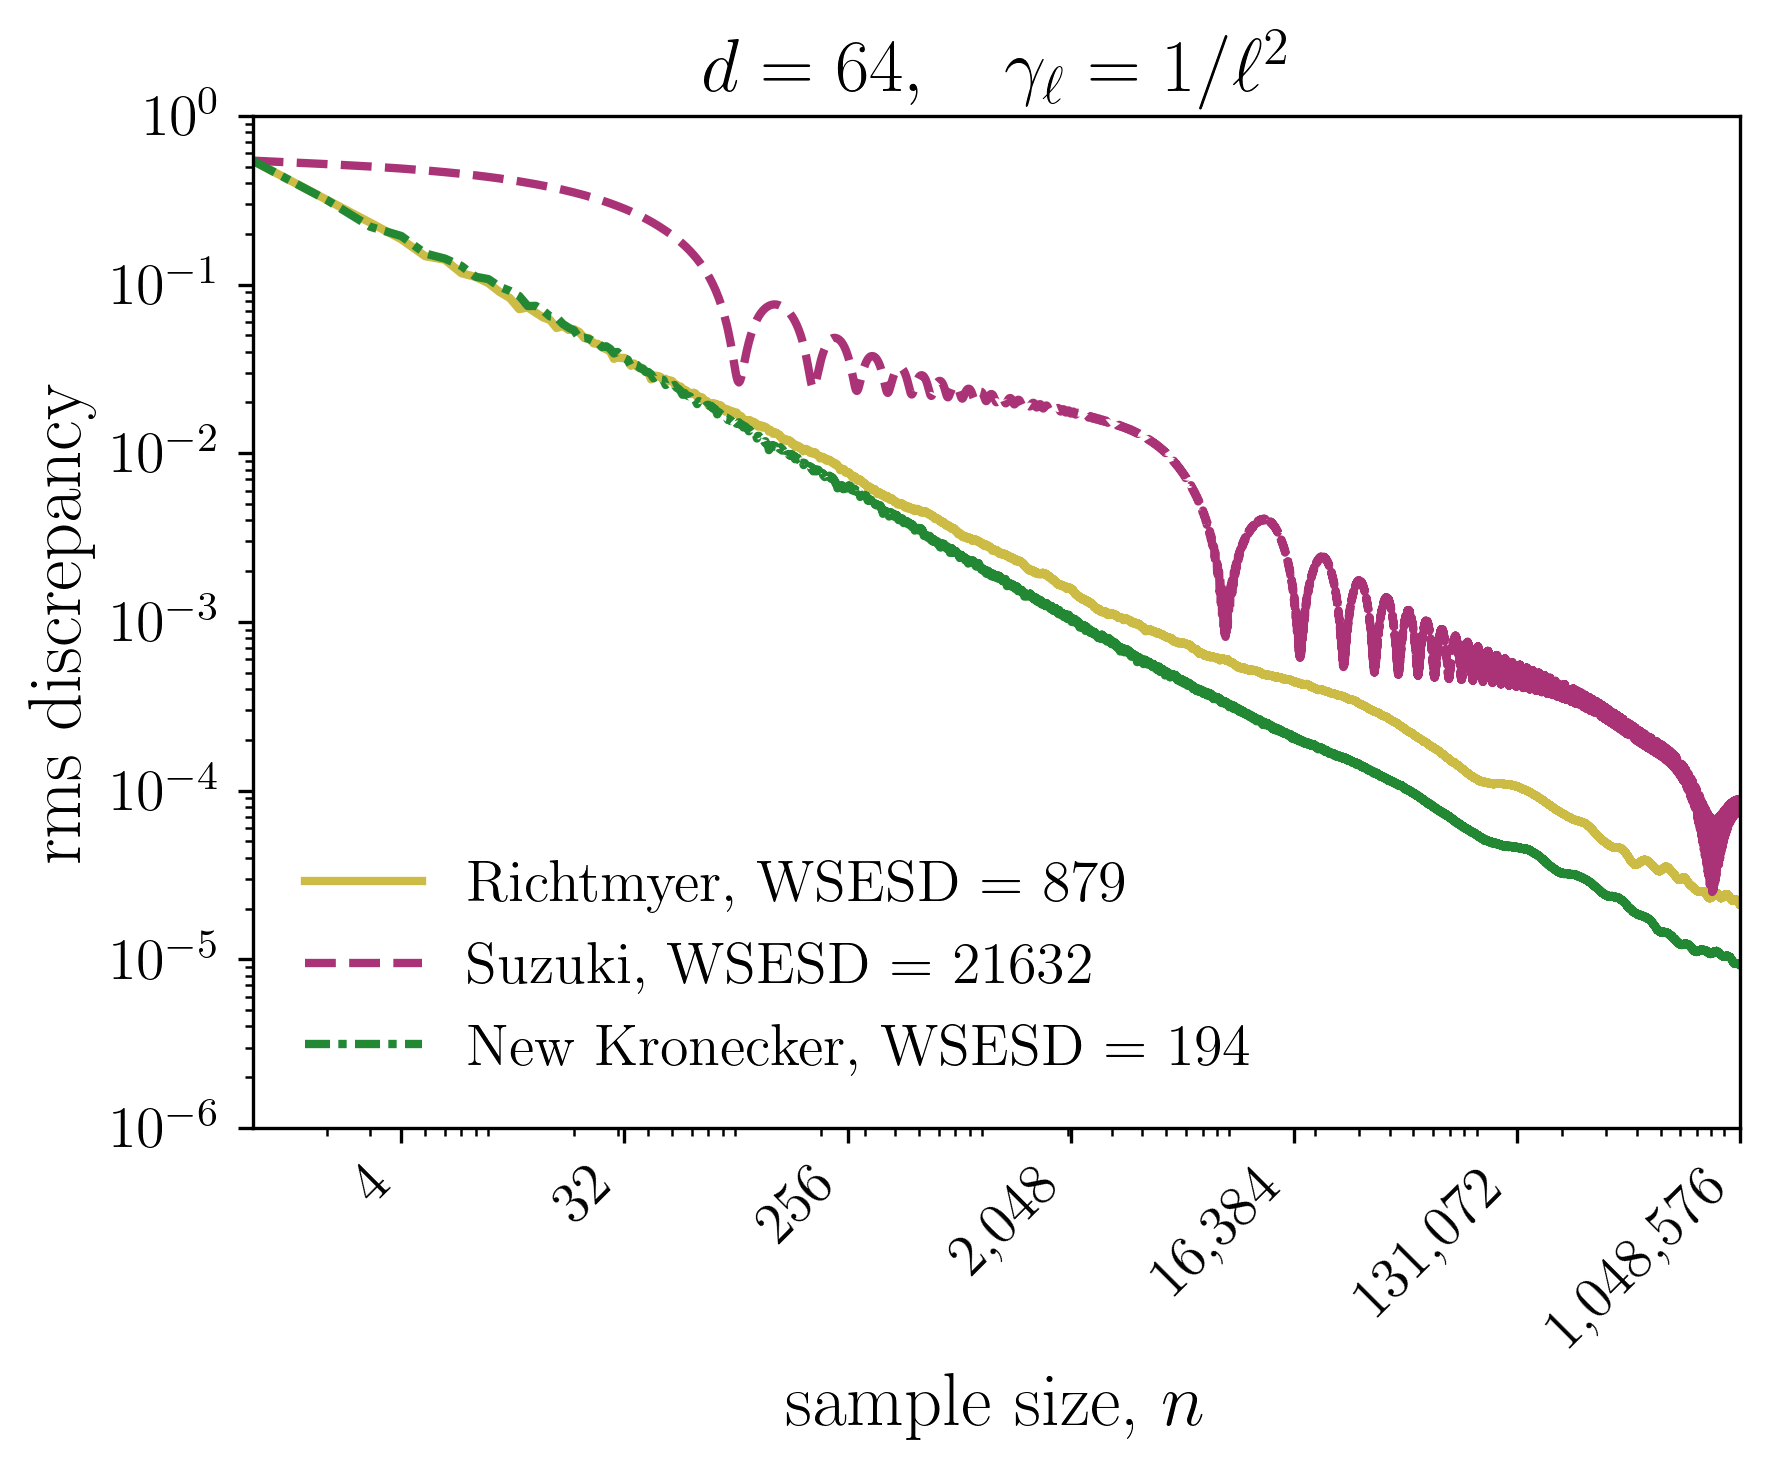
\includegraphics[width=.74\linewidth]{../../notebooks/artifacts/figures/special_d64_kronecker_discrepancy.png}
 \caption{Historical slide illustrations of root expected squared discrepancy:
 lattice sequences (top) and Kronecker sequences (bottom), with $d=64$,
 $N=2^{20}$, $\gamma_j=j^{-2}$, and $w_n=n$. The legends' aggregate values
 are inherited notebook outputs, not newly validated measurements.
 See the accompanying source-provenance record before using them as final results.}
 \label{fig:historical-cbc}
\end{figure}

The initial comparison motivates a more targeted experiment: improvement at
powers of the base need not coincide with improvement of the sum over all
prefix lengths. Conversely, a small aggregate criterion does not imply that
one sequence is best at every $n$. The final experiments should report both
$\W_N$ and the prefix-discrepancy curves, with preferred sample sizes marked,
under the same kernel, weights, and construction horizon.

To test Theorem~\ref{thm:newo-invariance}, fix a generating vector and
compare the original order with several random Newo maps on a finite dyadic
grid. Enumerate scalar pair-difference counts directly, then compare every
prefix's shift-averaged discrepancy with the reduced formula and compare their
weighted sums. The theorem predicts equality for each realized Newo map;
only the uniform-shift expectation remains. For a particular fixed shift or
integrand, integration errors need not agree.

The Kronecker experiments should separately compare the historical CBC rule,
Anders's new rule, and the algebraic baselines. Record the candidate set,
precision, seeds, stopping criteria, generating vectors, construction times,
and software revisions. Start with direct pairwise checks at small $N$ before
using accelerated formulas or reporting large-$N$ results. No new experimental
results are claimed in this draft.

\par\smallskip
\noindent\codex{[Author verification: Revalidate the historical plots before submission. The notebook uses
historical lattice-search interfaces that are absent from the currently pinned
QMCPy source. Also verify that the Kronecker discrepancy routine evaluates the
unshifted differences $\fracpart{k\vz}$: applying a fresh random shift to those
arguments would not implement \eqref{eq:kron-esd}. Inspect the code revision
actually used for the historical figures before drawing a conclusion about
their numerical validity. Agree on the new comparison of CBC methods: common
horizons and weights, intermediate versus preferred sample sizes, construction
costs, and a representative integration example if it fits the page budget.]}
\par\smallskip
